%!TEX root=../main.tex
\chapter{Projektmanagement}
Aufgrund der zeitlichen Befristung und der erheblichen Komplexität von \textit{Refundable} ist es notwendig, eine passende Projektmanagementmethode zu wählen. Zuerst gilt es aber zu klären, was der Begriff \Gls{pm} überhaupt bedeutet.\\
\begin{center}
	\textit{\enquote{Das \Gls{pm} umfasst die Führungsaufgaben, -organisation, -techniken und -mittel zur erfolgreichen Abwicklung eines Projekts. Die DIN 69901 definiert Projektmanagement als Gesamtheit von Führungsaufgaben, -organisation, -techniken und -mittel für die Abwicklung eines Projekts. Allgemeiner definiert das \Gls{pmi} im \Gls{pmbok} \Gls{pm} als Anwendung von Wissen, Fähigkeiten, Methoden und Techniken auf die Vorgänge innerhalb eines Projekts}}\cite{pm-definition}.
\end{center}
Das Projektteam hat während seiner Zeit am TGM im Rahmen des Unterrichts für \Gls{itp} vor allem mit der traditionellen Methode, dem Wasserfallmodell, und den zwei agilen Methoden Scrum und Kanban gearbeitet. Daher wird der Fokus nachfolgend auf diese Methoden gelegt.
\newpage
\section{Traditionelles Projektmanagement}
\label{chapter:tradi-pm}
Das traditionelle Projektmanagement hat einen linearen Ablauf. Das heißt, man notiert sich alle Aufgaben, die man abzuarbeiten hat und arbeitet sie alle der Reihe nach ab. Keine neue Aufgabe wird angefangen, bis diejenige davor abgearbeitet ist. Ein sehr wichtiger Punkt in diesem Managementsystem ist die viele Dokumentation, ohne die das System nicht funtkioniert. Verkörpert wird dieses Verfahren durch das Wasserfallmodell:
\begin{figure}[H]
	\centering
	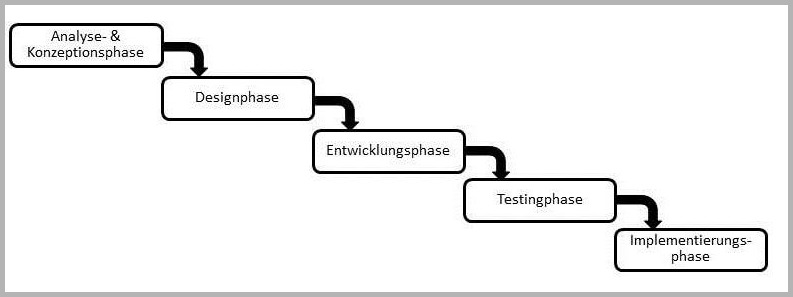
\includegraphics[width=0.7\linewidth]{images/projektmanagement/wasserfallmodell}
	\caption[Wasserfallmodell]{Illustration des Wasserfallmodells \cite{pm-wasserfall-online}}
	\label{fig:wasserfall}
\end{figure}
\subsection{Analyse und Konzeptionsphase}
In dieser Phase wird das Lastenheft und ein Projektstrukturplan erstellt, welche die groben Anforderungen des Projektes verkörpern. Danach wird die Machbarkeit (Grobanforderungen, Kosten, Ertrag, Realisierbarkeit, Umfeldanalyse, Projektorganisation, etc.) des Projektes mittels einer Machbarkeitsstudie analysiert \cite{pm-wasserfall-ionos}. In der Anforderungsdefinition, werden alle möglichen Funktionen definiert, die das Software-Projekt beinhalten soll und kann. Diese werden im Pflichtenheft notiert, auch Fachspezifikationen, oder Blueprint genannt. Alljene Dinge, die in der \textit{Analysephase} nicht bedacht werden, können im Laufe des Projektes gravierende Folgen auslösen \cite{pm-wasserfall-online}.
\subsection{Designphase}
Die \textit{Designphase} wird streng in Kundenkontakt durchgeführt \cite{pm-wasserfall-online} und ist dafür da, dass ein konkreter Lösungsvorschlag mit den definierten Anforderungen ausgearbeitet wird \cite{pm-wasserfall-ionos}. Es wird eine detaillierte Anleitung für die Erstellung der Software verfasst, die sich vor allem auf Komponenten wie Schnittstellen, Frameworks oder Bibliotheken bezieht. Als Resultat dieser Phase erhält man ein Entwurfsdokument mit Software-Bauplan, bzw. eine technische Spezifikation, als auch Testplänen, die sich auf einzelne Komponenten beziehen.
\subsection{Entwicklungsphase}
In dieser Phase, werden die in der \textit{Designphase} entwickelten Konzepte und Spezifikationen umgesetzt. Der Projektleiter spielt hier eine tragende Rolle, denn er muss sich bei aufkommenden Fragestellungen um externe als auch interne Probleme kümmern und in Kontakt mit dem Auftraggeber bleiben \cite{pm-wasserfall-online}. 
\subsection{Testphase}
In der \textit{Testphase} wird das Ergebnis der Entwicklungsphase getestet und auf Fehler geprüft \cite{pm-wasserfall-online}. Sollten diese auftreten werden sie ausgebessert und einem \textit{Re-Test} zugeführt, bis der Kunde das angefragte und funktionierende Endprodukt hat.
\subsection{Implementierungsphase}
In der \textit{Implementierungsphase} findet der \textit{Rollout} statt, welcher mittels einem \textit{Rolloutplan}, der bereits in der \textit{Designphase} erstellt wurde, durchgeführt wird \cite{pm-wasserfall-online}. Sollte es sich bei dem Projekt um Erweiterungen für eine bestehende Applikation handeln, dann sollte der \textit{Rollout} nicht zu \textit{Peakzeiten} stattfinden.
\section{Agiles Projektmanagement}
\label{chapter:agil-pm}
In agilen Methoden steht vor allem die Funktionalität im Vordergrund und nicht die Dokumentation, wie im traditionellen System \cite{pm-agil-ursula}. Durch die kurzen Iterationen haben Entwickler und Kunden ein besseres Gefühl für das entstehende Produkt und die Kundenwünsche können besser eingebaut werden. Alle agile Methoden sind Vorgehensmodelle, die von einem Wertekanon auf Prinzipien und Praktiken beruhen \cite{pm-agil-ursula}. 
\begin{center}
	\textit{\enquote{Agiles Projektmanagement bezeichnet Vorgehensweisen, 
			bei denen das Projektteam über hohe Toleranzen bezüglich Qualität, Umfang, Zeit und Kosten verfügt und eine sehr hohe Mitwirkung des Auftraggebers bei der Erstellung des Werks erforderlich ist. Charakteristisch für agiles Projektmanagement ist die Fokussierung auf das zu liefernde Werk und die Akzeptanz durch die Anwender. Hingegen werden geschäftliche Anforderungen, wie z. B. die Termintreue, Kostentreue oder Erfüllung eines spezifzierten Leistungsumfangs weniger oder nicht berücksichtigt}}  \cite{pm-agil-magazin}.
\end{center}
\subsection{Scrum}
Scrum ist ein empirisches Vorgehen, das in sogenannte \textit{Sprints} (ein zeitlich begrenztes Event) eingeteilt ist \cite{pm-agil-ursula}. Ein \textit{Sprint}, besteht aus dem \textit{Sprint Planning}, in dem der kommende, maximal vier wöchige \textit{Sprint}, geplant und durchgesprochen wird. Genauer gesagt werden Aufgaben von dem \textit{Project Backlog} (Der Wunschliste, des Kunden), in den \textit{Sprint Backlog} (die Aufgaben, die das \textit{Development Team} in einem Sprint durchführen wird) verschoben. Jeden Tag im \textit{Sprint} gibt es einen \textit{Daily Scrum}, in dem ein 15 minütiges \textit{Standupmeeting} stattfindet. Dieser Ablauf ist grafisch in \autoref{fig:scrum} dargestellt.
\begin{figure}[H]
	\centering
	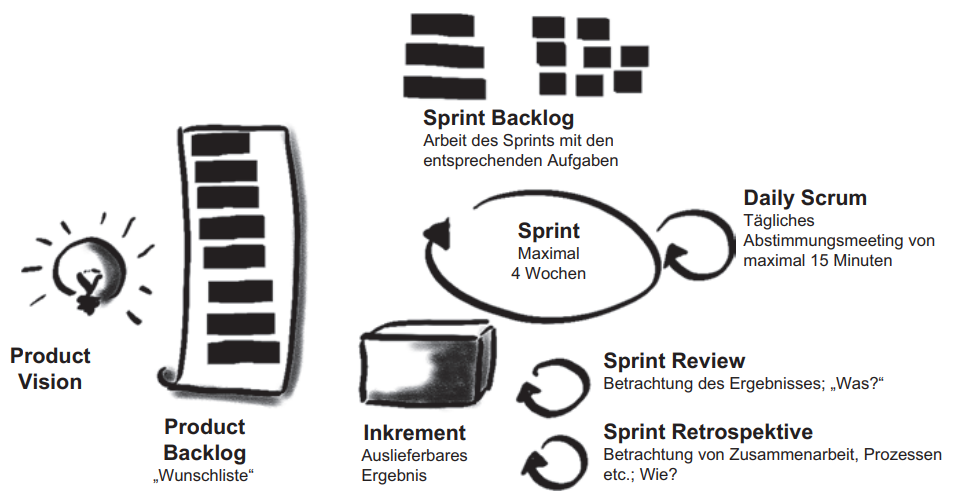
\includegraphics[width=0.6\linewidth]{images/projektmanagement/scrum2}
	\caption[Scrum]{Illustration Scrum \cite{pm-agil-ursula}}
	\label{fig:scrum}
\end{figure}
\subsubsection{Scrum-Rollen}
\paragraph{Product Owner}~\\
Der \textit{Product Owner} trägt die Verantwortung des Produktes. Üblicherweise bringt dieser ein ausgebrägtes Branchenwissen mit sich, das den Erfolg und die Profitabilitär des Produktes garantieren soll.
\paragraph{Scrum Master}~\\
Der \textit{Scrum Master} hilft dem \textit{Development Team} dabei, wie man spezielle Herausforderungen lösen kann. Seine Hauptaufgabe ist es, sich um die Scrum-Werte und Methoden und die Prozesse zwischen den verschiedenen Rollen zu kümmern.
\paragraph{Development Team}~\\
Das \textit{Development Team} setzt die \textit{Tasks} selbstständig um und erstellt die aus den \textit{Sprints} resultierenden Produktinkremente, die jeweils testbare Einheiten bilden sollten und im Anschluss getestet werden.

\subsection{Kanban}
In \textit{Kanban} gibt es keine bestimmten Rollen, die den Projektmitglieder zugewiesen werden, wie in Scrum \cite{pm-agil-ursula}. Es gibt ein \textit{Kanban-Board}, welches einen strukturierten Aufbau, von Links nach Rechts beinhaltet. Alle Aufgaben aus dem \textit{Backlog} werden als sogenannte \textit{To do's} ganz Links angezeigt. Des Weiteren gibt es eine Spalte, in der die Aufgaben gesammelt werden, die als Nächstes behandelt werden. Dieses Verfahren wird, bis zu der Spalte fortgeführt, in welcher die abgeschlossenen \textit{To do's} gesammelt werden. Der Ablauf dieser Spalten ist ähnlich inkrementell, wie bei \textit{Scrum}. Jedoch werden die Arbeitspakete nicht zugeteilt, sondern das \textit{Development Team}, zieht sich die \textit{Tickets} selbstständig (auch unter dem Begriff \textit{Pull-Prinzip} bekannt). Siehe \autoref{fig:kanban} zur Veranschaulichung des \textit{Kanban-Boards}. 
\begin{figure}[H]
	\centering
	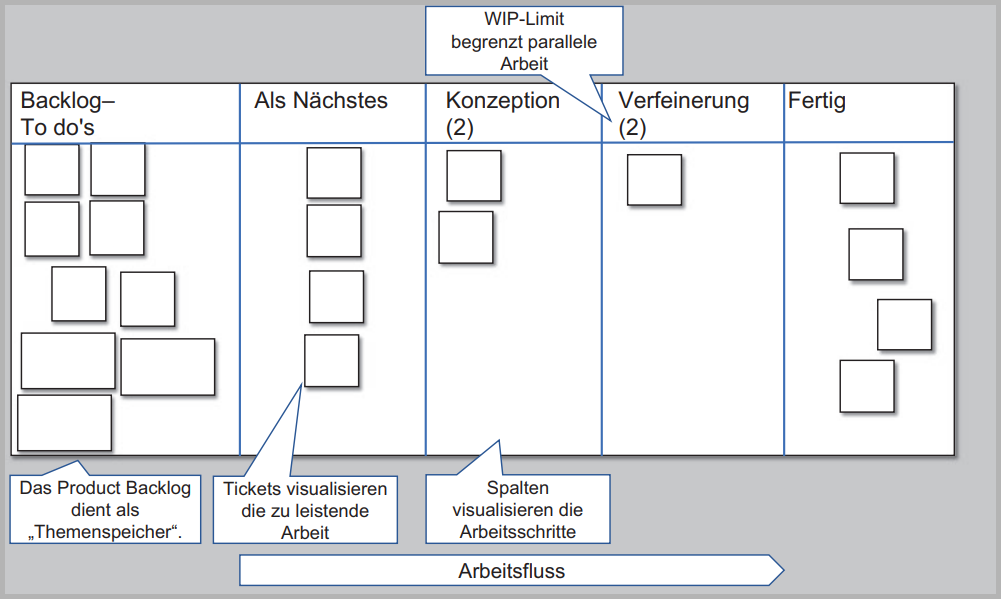
\includegraphics[width=0.6\linewidth]{images/projektmanagement/kanban}
	\caption[Kanban]{Illustration Kanban \cite{pm-agil-ursula}}
	\label{fig:kanban}
\end{figure}
\section{Fazit}
Angesichts des hohen Dokumentationsaufwandes im traditionellen Projektmanagement, hat sich das Team einerseites, wegen des Fokuses, auf das Endprodukt für eine agile Methode entschieden. Da \textit{Kanban} im Gegensatz zu \textit{Scrum} nicht disruptiv, sondern evolutionär ist und man daher keine neuen Rollen zuweisen muss, hat sich das Projektteam für \textit{Kanban} entschieden, nicht zuletzt ob des geringen Implementierungsaufwandes. Ein weiterer Entscheidungsgrund war, dass das Projektteam parallel zu ihren schulischen Aktivitäten arbeiten muss und gleichmäßige Sprints nicht garantiert möglich sind. Ebenfalls hat die Integration, des \textit{Kanban-Boards} in \textit{GitHub}, die Entscheidung für \textit{Kanban} beeinflusst.